\documentclass{article}
\usepackage[utf8]{inputenc}
\usepackage{amsmath}
\usepackage{amsthm}
\usepackage{amsfonts}
\usepackage{amssymb}
\usepackage{amstext}
\usepackage{gensymb}
\usepackage{graphicx}
\usepackage{enumerate}
\pagenumbering{arabic}
\usepackage{fancyhdr}
\usepackage[margin=0.75in]{geometry}
\usepackage{eucal}
\usepackage{parskip} % removes auto indentation for paragraphs
\usepackage{enumitem} % changes the indexing for enumerate
\setlist[enumerate,1]{label = {(\alph*)}}

\usepackage{mathtools} % used for making a ceiling function

\DeclarePairedDelimiter{\ceil}{\lceil}{\rceil} %create ceiling function as \ceil{x}, \ceil*{x} to add \left and \right

\usepackage{listings} % import code into latex

\usepackage{algorithm} % used to write algorithms
\usepackage[noend]{algpseudocode}

\def\N{\mathbb{N}}
\def\Z{\mathbb{Z}}
\def\Q{\mathbb{Q}}
\def\R{\mathbb{R}}
\newcommand{\Mod}[1]{\ (\text{mod}\ #1)}
\newcommand{\Problem}[1]{\textbf{Problem #1}}
\newcommand{\li}[0]{\liminf_{n\to\infty}}
\newcommand{\ls}[0]{\limsup_{n\to\infty}}
\newcommand{\dl}[2]{\displaystyle\lim_{#1 \to #2}}
\newcommand{\ds}[2]{\displaystyle\sum_{#1}^{#2}}
\newcommand{\ra}{\Rightarrow}

\linespread{1.5}

\usepackage{float}

\title{CSE 6140 - Homework 1}
\author{Alexander Winkles}
\date{}


\begin{document}

\maketitle

\vspace{2in}

For assignment 1, I worked with Willian Kong on several problems. 
I utilized the class textbooks (Kleinberg, CLRS, and Benoit) as well as the website ``GeeksForGeeks'' for different perspectives on designing the algorithms.
Overall, I enjoyed this assignment.
However, I still feel uncomfortable proving optimality of algorithms, so more practice and examples with that would be appreciated!
Additionally, I think the size of the graph files for the final problem were a bit too large.
Once the first few graphs were solved, I think it became unnecessary to keep analyzing more, as we knew our algorithm worked. 

\newpage

\Problem{1}

\begin{enumerate}

% https://tex.stackexchange.com/questions/163768/write-pseudo-code-in-latex
\item Let $k \geq \ceil{\log{n}}$. 
We wish to design an algorithm of complexity $O(\log{n})$.
This suggests the idea of an algorithm similar to the methodology behind the Bisection Method.
\begin{algorithm}[H]
\caption{Bisection Search for Box Dropping}
\begin{algorithmic}[1]
\Procedure{BisectionSearch}{$l,n$}
\State $j \gets n$ \Comment{Highest Floor}
\State $i \gets l$ \Comment{Lowest Floor}
\State $m \gets \frac{i + j}{2}$
\If {$m = \text{break}$} \Comment{Checks if box breaks on floor m}
\State \Call{BisectionSearch}{$1,m-1$}
\Else
\State \Call{BisectionSearch}{$m,n$}
\EndIf
\Return {$m$}
\EndProcedure
\end{algorithmic}
\end{algorithm}
The nature of the algorithm guarentees that this algorithm will take at most $\log{n}$ steps, so we will not run out of boxes.

\item Let $k < \ceil{\log{n}}$.
We wish to design an algoirthm of complexity $O(k + \frac{n}{2^{k-1}})$.
To accomplish this, we will use the bisection search from above, but only using $k-1$ boxes rather than $k$.
The last box will then search the remaining interval by going up each floor and throwing the final box off. 
Because of this methodology, there will be at most $n/2^{k-1}$ floors in the interval, leading to the desired complexity of $O(k + n/2^{k-1})$.

\item Let $k = 2$. 
We wish to design an algorithm of complexity $O(\sqrt{n})$. 
\begin{algorithm}[H]
\caption{Box Dropping for $k = 2$}
\begin{algorithmic}[1]
\Procedure{FloorSearch}{$n$}
\State $m \gets 0$ \Comment{Initializes maximum floor}
\State $Nstep \gets \sqrt{n}$ \Comment{Number for floors to iterate over}
\For {$i = 1:n:Nstep$}
\State \If {$i \neq \text{break}$}
\State $m \gets i$
\State $\textbf{break}$
\EndIf
\EndFor
\For {$i = m+1:m+\sqrt{n}$}
\State \If {$i \neq \text{break}$}
\State $m \gets i$
\State $\textbf{break}$
\EndIf
\EndFor
\Return {$m$}
\EndProcedure
\end{algorithmic}
\end{algorithm}

\end{enumerate}

\Problem{2}

\begin{algorithm}[H]
\caption{Greedy 1}
\begin{algorithmic}[1]
\Procedure{MinimizeStrips}{$C,n$}
\State $m \gets 1$ \Comment{number of strips needed}
\State $\textbf{Sort}\text{ nodes $c_i$ from leftmost to rightmost so that $c_1 < c_2 < \hdots < c_n$}$
\State $minNode \gets c_1$ 
\For {$i = 1:n$}
\If {$c_i - minNode > 9$}
\State $m \gets m+ 1$
\State $minNode \gets c_i $
\EndIf
\EndFor
\State \Return {$m$}
\EndProcedure
\end{algorithmic}
\end{algorithm}

Essentially, this algorithm works by sorting all the nodes (``holes'') from left to right.
From here, it starts at the leftmost strip then adds other nodes that will fit within the 9 inches of strip.
Once all the nodes for a strip are filled, a new strip is added to the next node and the process is repeated.
Given that this has a single for loop, its time complexity is $T(n) \in O(n)$.

Consider the subproblem of several nodes clustered together in such a way that there is no more than 9 inches between the leftmost and rightmost nodes.
With our greedy choice, this subproblem will be covered completely by a single strip, which is trivially optimal.
Thus, as the algorithm will treat all such subproblems this way, we can inductively see that the algorithm is optimal.

\Problem{3}

\begin{algorithm}[H]
\caption{Greedy 2}
\begin{algorithmic}[1]
\Procedure{MaximizeValue}{$L, M$}
\State $\text{weightUsed} \gets 0$
\State $B \gets \emptyset$
\State \textbf{sort} minerals $m_i$ by $\frac{v_i}{w_i}$ from highest value to lowest
\For {$m_i \in M$}
\If {$\text{weightUsed} + w_i \leq L$}
\State $B = B \cup \{m_i\}$
\State $\text{weightUsed} + w_i$
\State $M = M - \{m_i\}$
\State \textbf{break}
\EndIf
\EndFor
\If {$\text{weightUsed} < L$}
\State pick the mineral next in line in $M$ and call it $m$, with weight of $w$ and value of $v$
\State $B = B \cup \{m * \frac{w}{L - \text{weightUsed}}\}$
\EndIf
\State \Return {$B$}
\EndProcedure
\end{algorithmic}
\end{algorithm}


In order for this algorithm to be optimal, the bag must be completely filled in order to maximize profits.
\newtheorem{bag}{Theorem}
\begin{bag}
The bag has been completely filled by the algorithm.
\end{bag}
\begin{proof}
This result is easy to see. 
At the end of the for loop, there are two possibilities: 
\begin{enumerate}
\item weightUsed $ = L$
\item weightUsed $< L$
\end{enumerate}
If it is the first case, we are done.
However, if it is the second case, then we can fit $L - \text{weightUsed}$ amount into the bag.
Our algorithm provides this by adding a portion of the next mineral scaled with weight $L - \text{weightUsed}$, so after this our bag is again full.
This completes our proof.
\end{proof}

\begin{bag}
The greedy algorithm is optimal.
\end{bag}
\begin{proof}
Consider an optimal algorithm $\mathcal{O}$.
Our goal is to use an exchange argument to show that the greedy solution $A$ is optimal.
Arrange the minerals in both as such in the algorithm, so $m_i$ is first if and only if $v_i / w_i$ is largest.
Consider every mineral $o_i$ in $\mathcal{O}$ that differs from $a_i$ in $A$.
We can exchange this mineral with the corresponding mineral in $A$. 
If they are of different weights, we can instead exchange it for the appropriate portion of $a_i$.
By definition of the greedy algorithm, $v_{a_i} \geq v_{o_i}$, where the equality holds otherwise $\mathcal{O}$ is not optimal.
By continuously exchanging minerals using the above procedure, we arrive at an optimal solution no worse that the one we started with that is identical to $A$, so thus $A$ must be optimal.
\end{proof}

\newpage

\Problem{4}

For this problem, I chose to implement Prim's algorithm in Python.
I chose this problem because it was the less intuitive of the two for me, so I thought that writing code for it would help me gain a better understanding.
Rather than designing a second algorithm for recomputeMST, I chose to instead append the new edge to my graph then run computeMST again.
Because I implemented a priority queue utilizing Python's heapq package, my complexity should theoretically be $O(m\log{n})$, where $n$ is the number of nodes and $m$ is the number of edges. 
\begin{figure}[H]
\centering
\begin{minipage}[b]{0.4\textwidth}
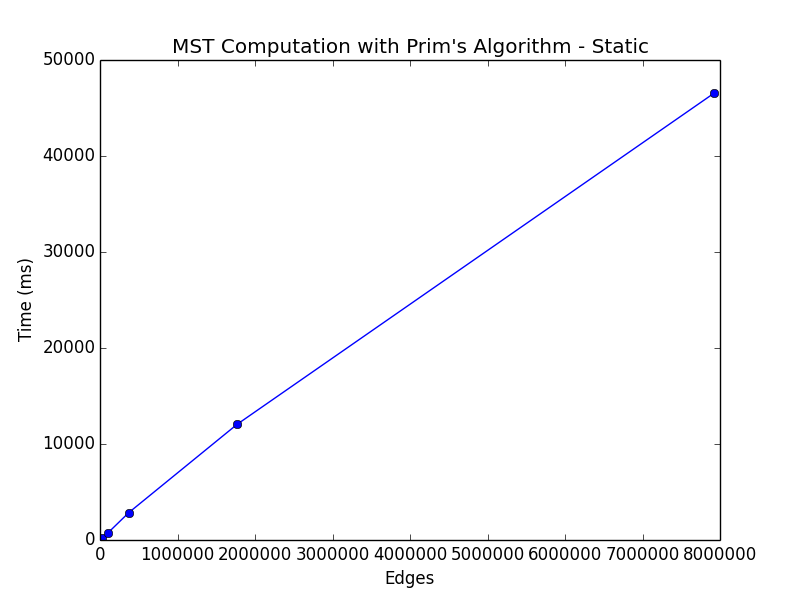
\includegraphics[height=7cm]{static}	
\end{minipage}
\hspace{0.6in}
\begin{minipage}[b]{0.4\textwidth}
\centering
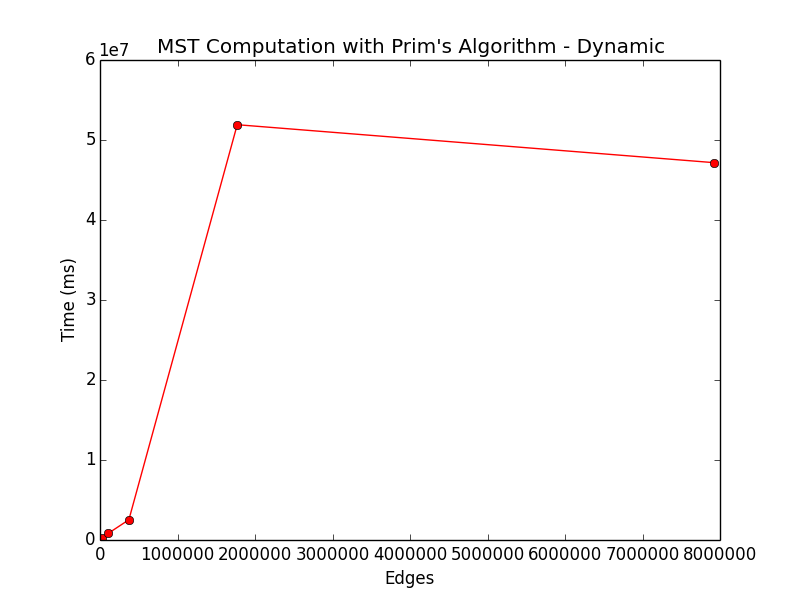
\includegraphics[height=7cm]{dynamic}	
\end{minipage}
\end{figure}
From the graphs above, the static computation appears to behave linearly with respect to the edges.
The dynamic, on the other hand, appears more akin to $m \log{n}$, which is expected given the theoretical complexity of Prim's algorithm. 
I assume the difference in the graphs can be justified by the addition of edges during the dynamic process. 
Since occasionally new edges are added to the graph, this increases the time it would take to calculate a single instance of Prim's, whihc leads to an overall increase in the time required to run the computation. 

\end{document}
